s\section{Descrizione procedura di ranging tra le ancore presente nel firmware originale}
\begin{frame}[shrink=10]{Introduzione}
  Nel seguito viene descritta, mediante un sequence diagram, la procedura di ranging tra le ancore
  presente nel firmware originale. Nel diagramma verrà utilizzata una terminologia similare a quella utilizzata nelle slide precedenti.\\
  Nella lettura del diagramma si tenga conto delle seguenti
  \begin{itemize}
  \item[-] i blocchi di colore bianco rappresentano stati della macchina a stati;
  \item[-] i blocchi di colore verde rappresentano le callback di ricezione;
  \item[-] nello schema presentato \alert{solo} le ancore A0 ed A1 inviano il Poll alle altre ancore
    non perché lo schema sia semplificato. Infatti il firmware originale prevede
    il calcolo di un numero di range tra le ancore limitato a $3$ (ossia $r01$, $r02$ ed $r12$);
  \item[-] si ricordi che la procedura di ranging tra le ancore originale viene eseguita negli ultimi
    due slot di ogni superframe;
  \item[-] \lstinline!TofArrayAnc! è la struttura dati in cui le ancore salavano i tof ricevuti;
  \item[-] \lstinline!A1 Slot Time! è un campo utilizzato dall'ancora A1 per decidere quando è il momento
    di inviare il Poll.
  \end{itemize}
  
\end{frame}

\begin{frame}{Modalità di Autoranging inclusa nel Firmware}  
  \begin{center}
    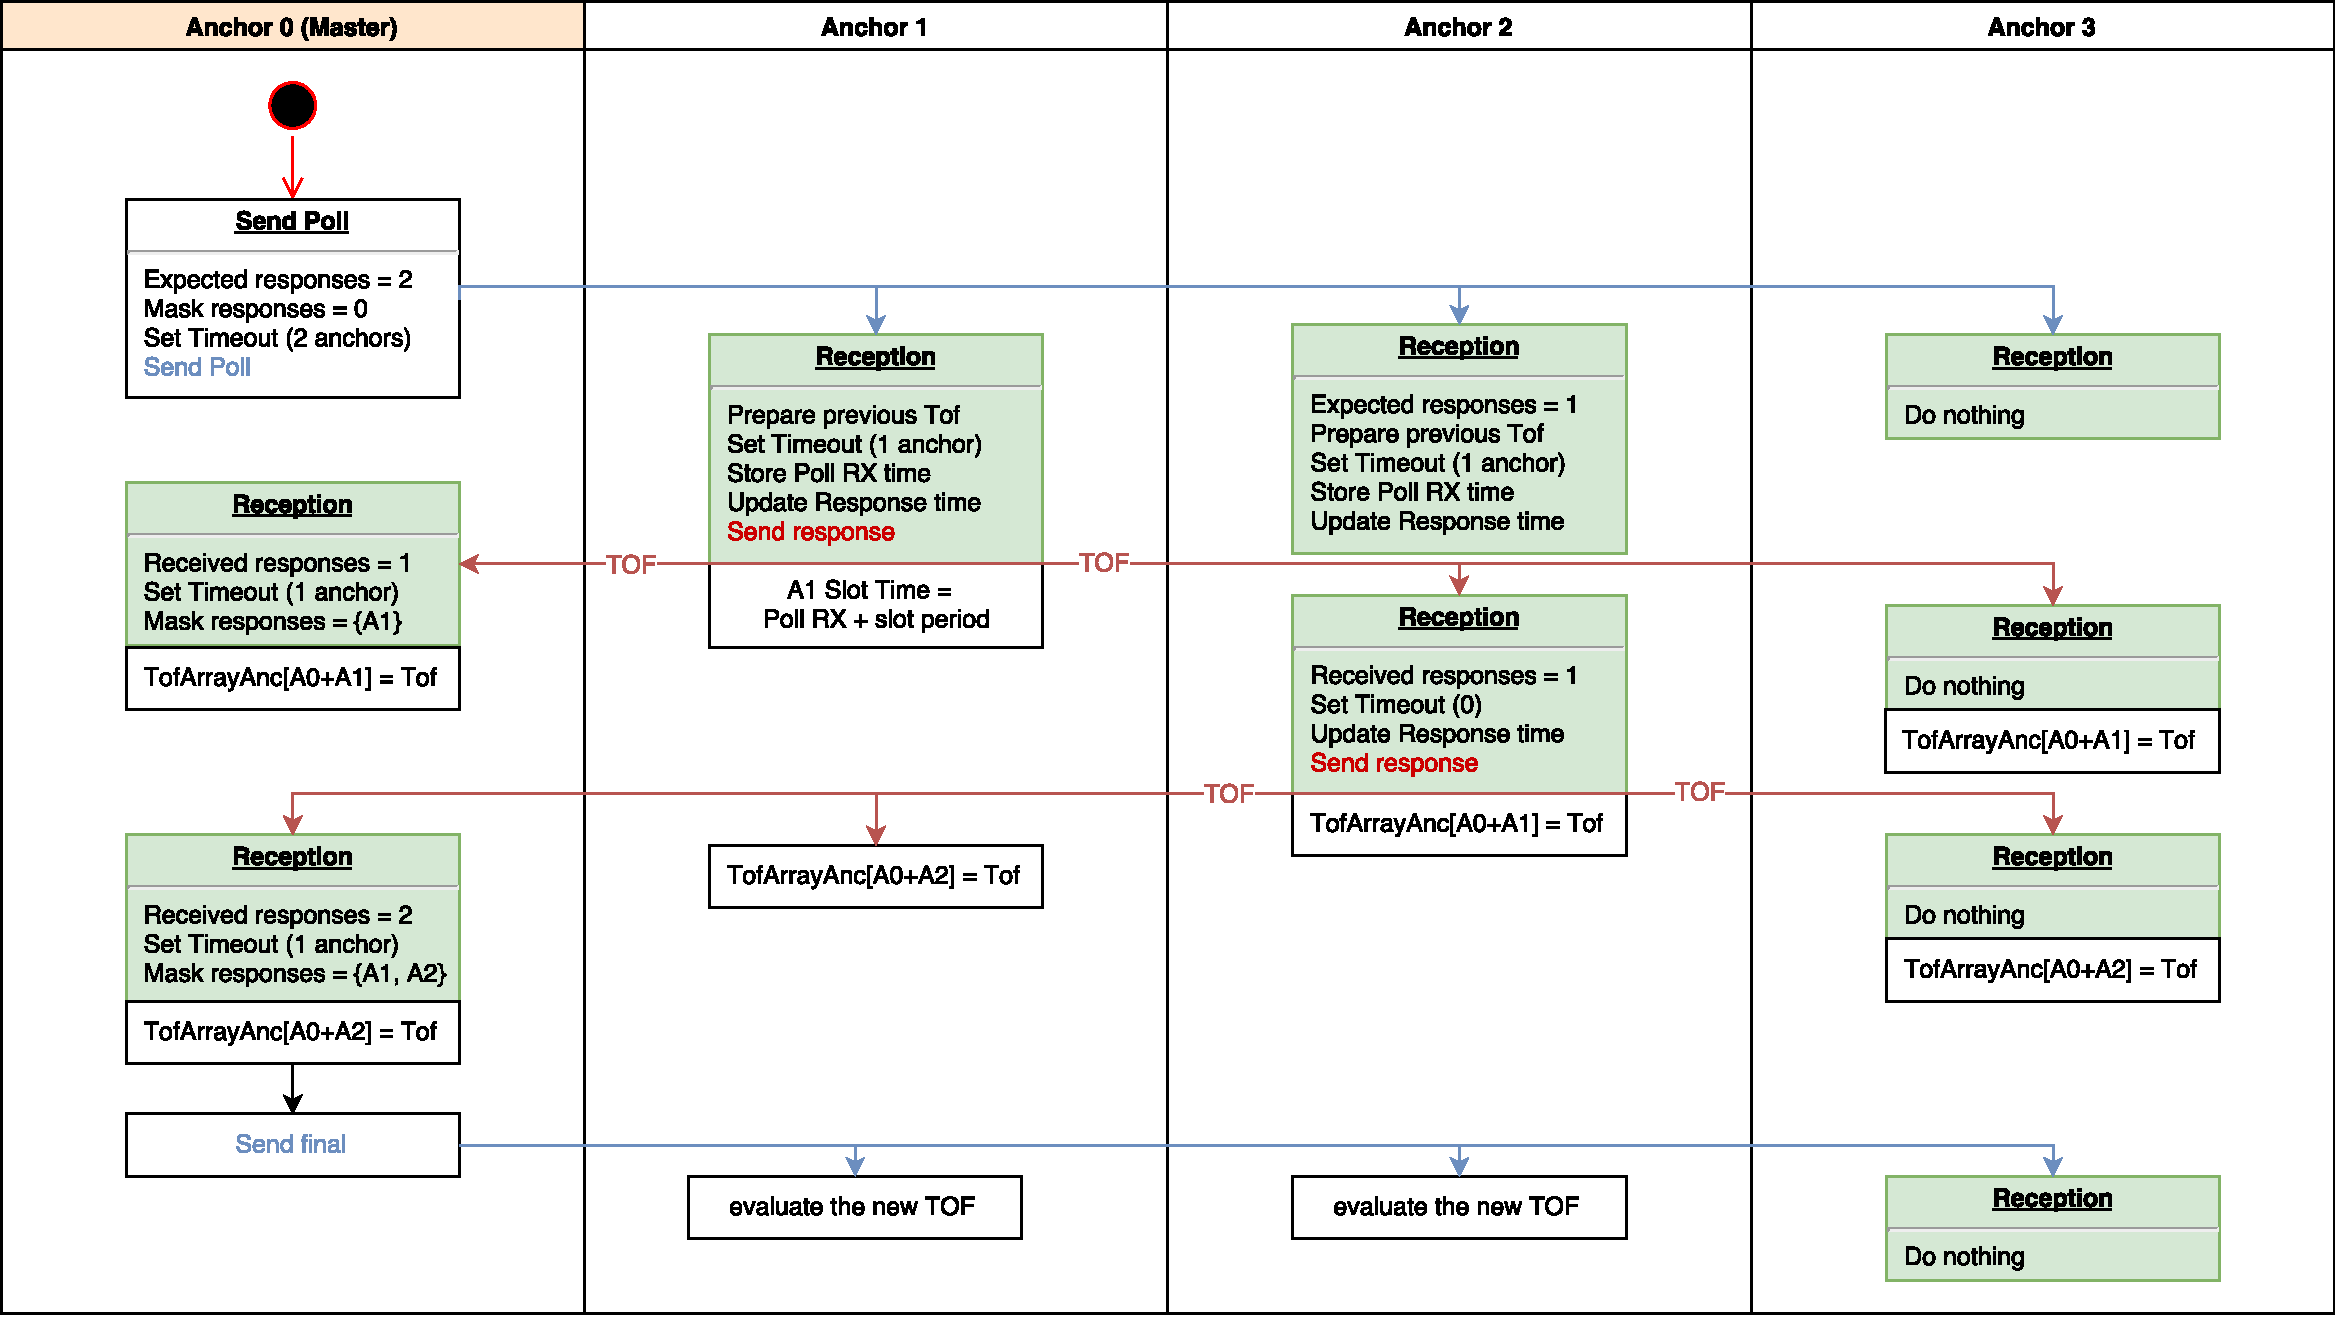
\includegraphics[width=\linewidth]{A2A_oldA0.pdf}
  \end{center}
\end{frame}

\begin{frame}{Modalità di Autoranging inclusa nel Firmware}
  \begin{center}
    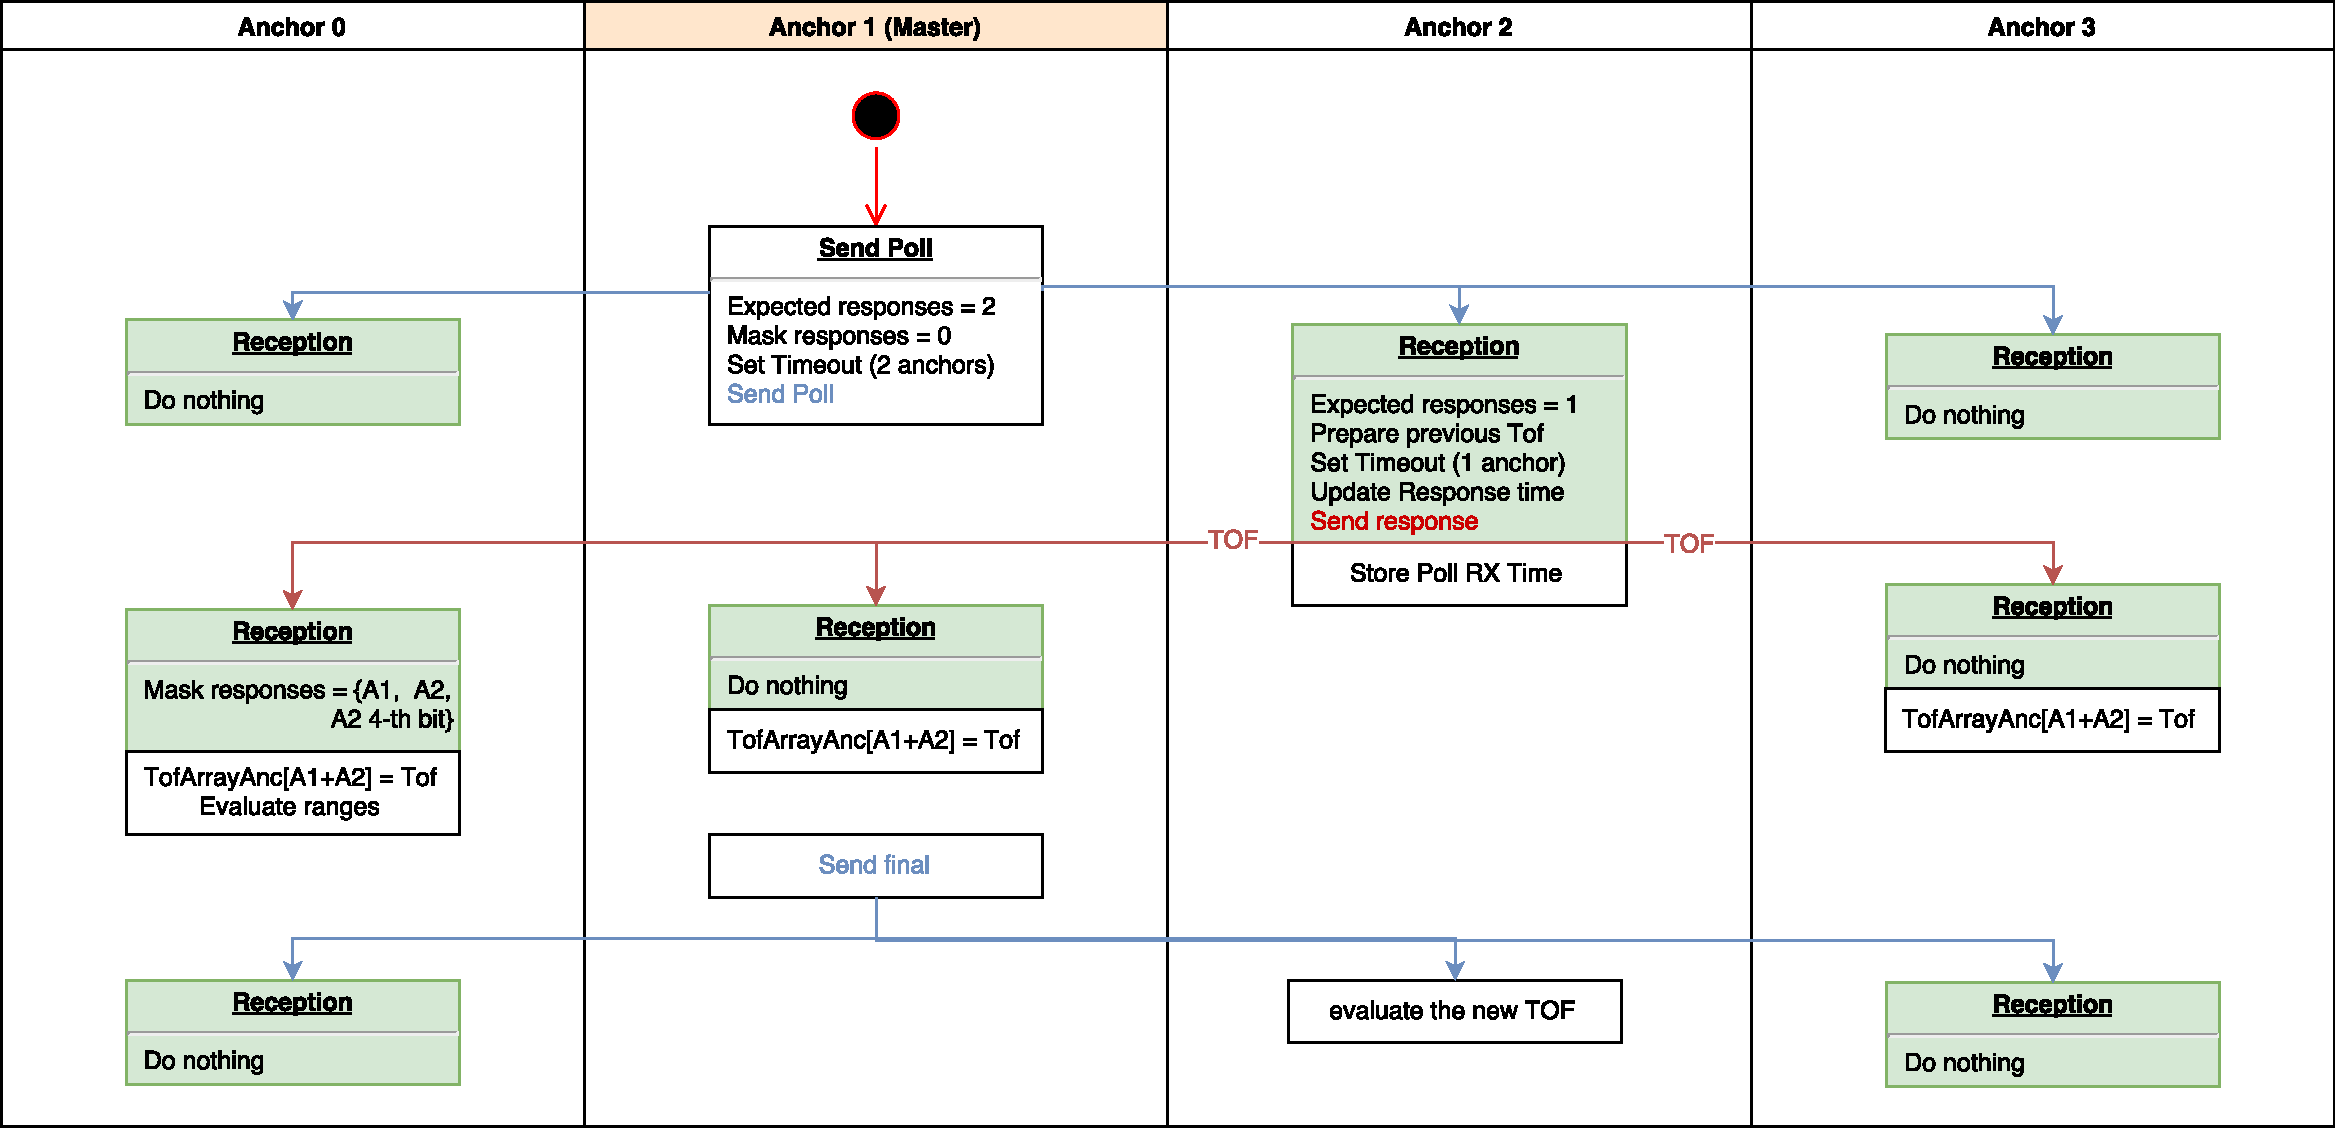
\includegraphics[width=\linewidth]{A2A_oldA1.pdf}
  \end{center}
\end{frame}

\begin{frame}{Considerazioni}
  La procedura presentata presenta le seguenti limitazioni:
  \begin{itemize}
  \item [-] calcola solo 3 su 6 dei range richiesti per valutare la posizione delle ancore;
  \item [-] non spedisce i range calcolati / la loro media ai tag;
  \item [-] è implementata mediante parti di codice specifiche per ogni ancora quindi \alert{non}
    facilmente estensibile al caso di più ancore.
  %\item [-] a parita di scelta del superframe period e dello slot period \alert{riduce} di $N$ il numero
  %  massimo di tag utilizzabili poiché la procedura avviene negli ultimi $N$\footnote{nel caso del
  %    firmware $N = 2$} slot.
  \end{itemize}
\end{frame}

\section{Nuova procedura di autoranging}

\begin{frame}[shrink = 10]{Introduzione}
  A differenza della procedura originale la nuova procedura \alert{non} avviene periodicamente
  durante gli ultimi slot del superframe ma in una fase preliminare durante la quale il tag rimane in attesa.
  \par
  Nel dettaglio:
  \begin{itemize}
  \item [1.] Ogni ancora \alert{a turno} valuta $M$ volte i range di interesse, i.e. l'ancora
    j-esima raccoglie $M$ volte i range $r_{j,j+1}$ ... $r_{j,N-1}$ con $N$ il numero di ancore e $j<N$;
  \item [2.] Una volta che tutte le ancore hanno ottenuto le misure ciscuna calcola la media dei range raccolti;
  \item [3.] Mediante un meccanisco di time out il tag esce dalla fase di attesa ed inizia la normale procedura di ranging;
  \item [4.] ogni ancora, sfruttando il meccanismo di divisione temporale già descritto nella slide \ref{anchors_responses_turn},
    invia la risposta al tag contenente, oltre al tof, i range medi di interesse.
  \end{itemize}
\end{frame}

\begin{frame}{Simmetria}
  In linea di principio quando l'ancora j-esima esegua la sua fase di raccolta dei range non è
  necessario che le ancore con indice $i < j$ partecipino alla procedura poiché sono di interesse solo
  i range $r_{j,k}$ con $j < k < N$. Tuttavia facendo partecipare sempre tutte le ancore è possibile
  raccogliere per $M$ volte ciascun range eseguendo $M/2$ istanze di range per ogni ancora invece che $M$.

  \begin{exampleblock}{Numero di istanze di range richieste}
    Date $N$ ancore per raccogliere $M$ volte ciascun range di interesse sono richieste
    \[
    N \frac{M}{2}
    \]
    istanze di ranging
  \end{exampleblock}
\end{frame}

\begin{frame}{Simmetria - esempio}
  Sia $i<j$, l'ancora $A_i$ esegue $M/2$ istanze di ranging
  \begin{center}
    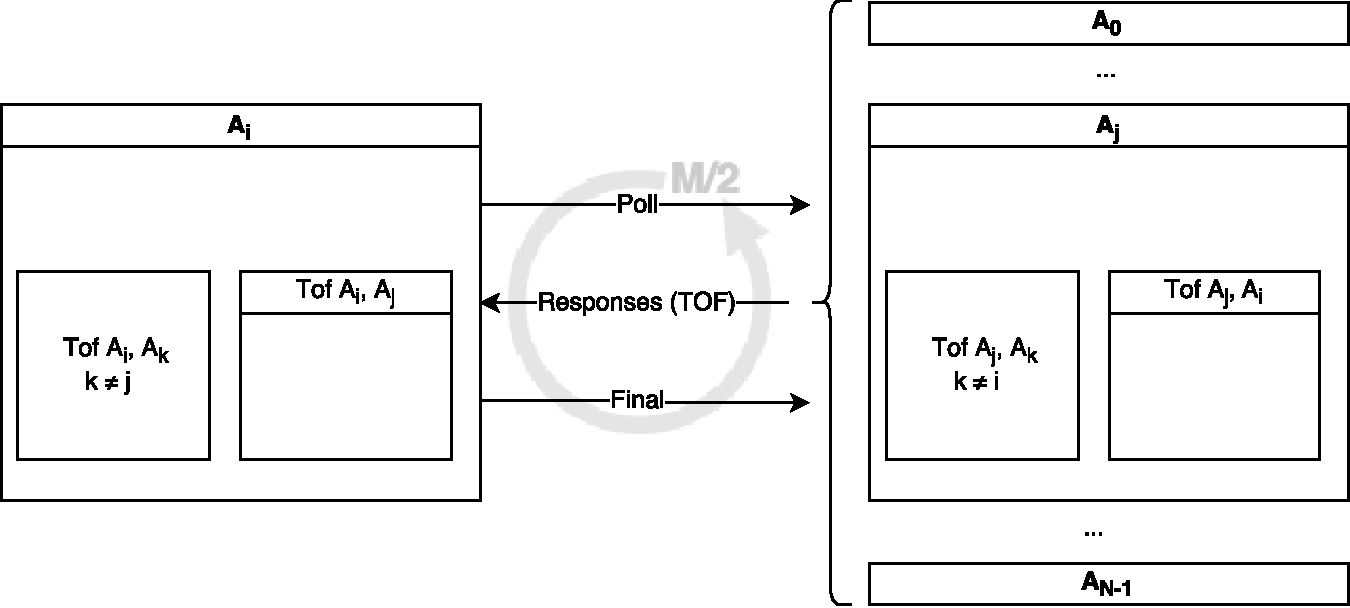
\includegraphics[width=\linewidth]{new_autoranging_1.pdf}
  \end{center}
\end{frame}

\begin{frame}{Simmetria - esempio}
  L'ancora $A_i$ ha memorizzato $M/2$ misure di ranging
  \begin{center}
    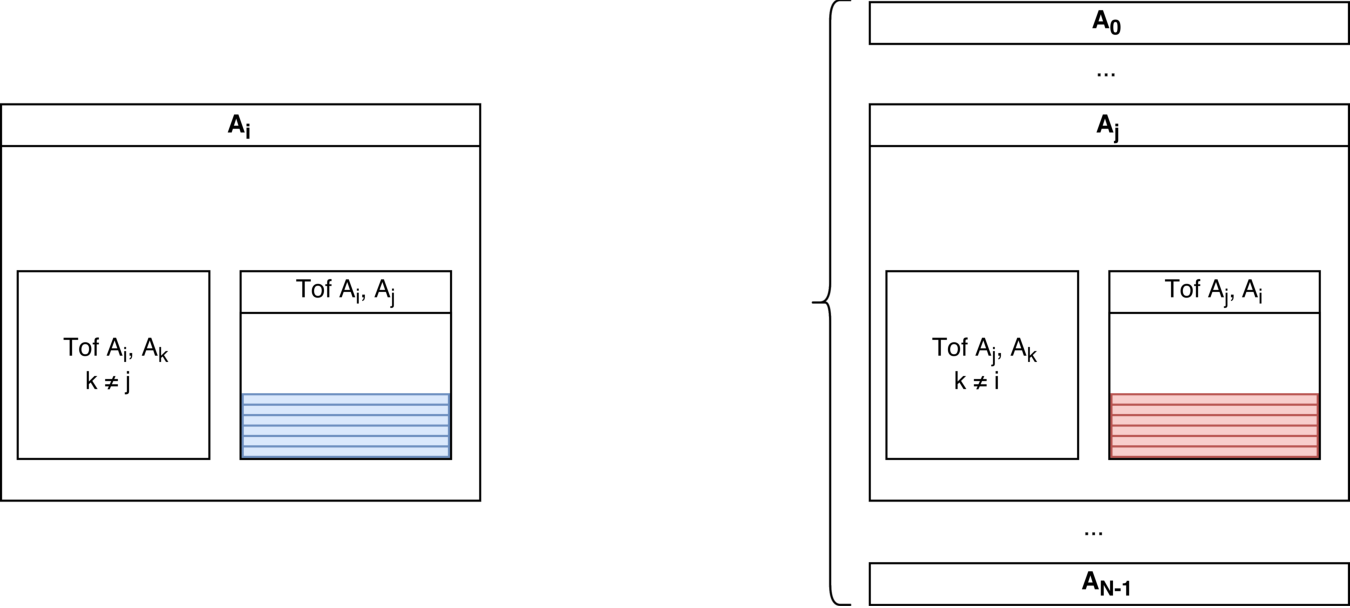
\includegraphics[width=\linewidth]{new_autoranging_2.pdf}
  \end{center}
\end{frame}

\begin{frame}{Simmetria - esempio}
  Successivamente l'ancora $A_j$ esegue $M/2$ istanze di ranging
  \begin{center}
    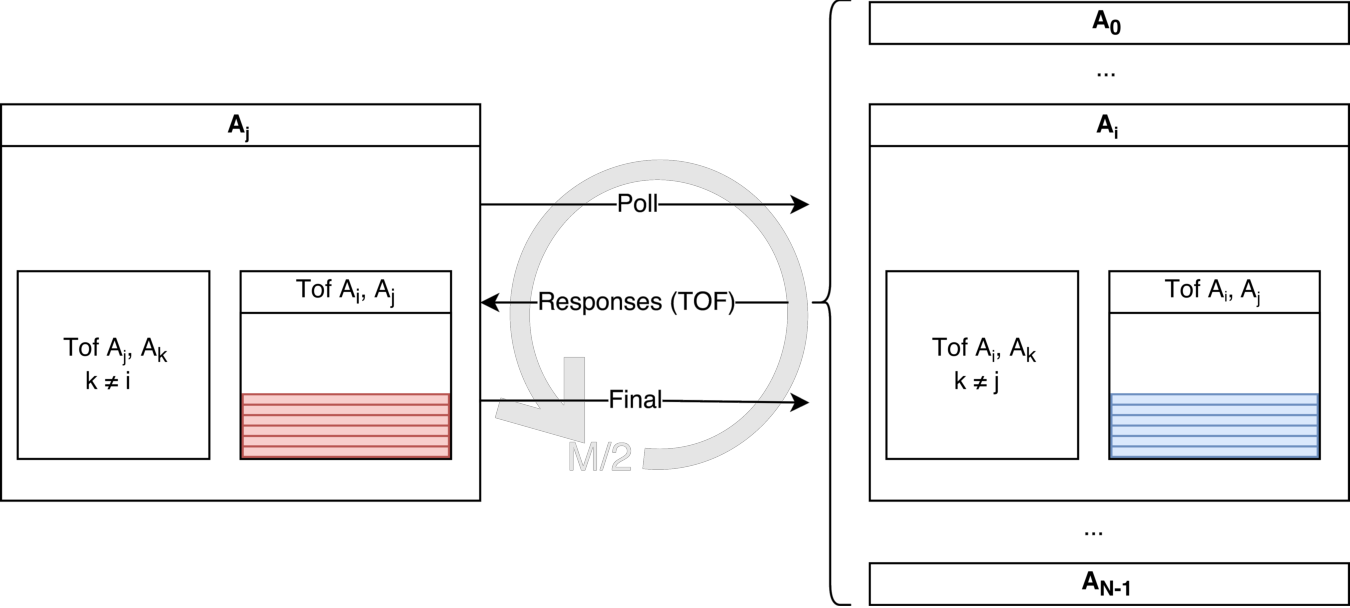
\includegraphics[width=\linewidth]{new_autoranging_3.pdf}
  \end{center}
\end{frame}

\begin{frame}{Simmetria - esempio}
  L'ancora $A_i$ colleziona ulteriori $M/2$ misure
  \begin{center}
    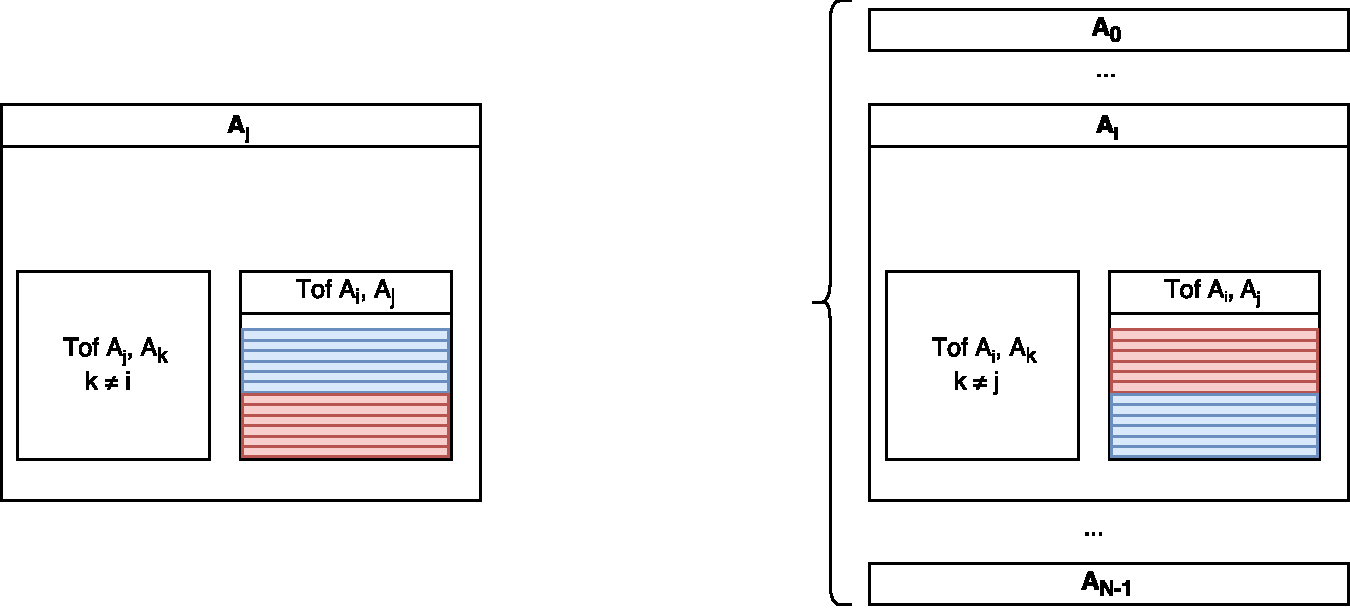
\includegraphics[width=\linewidth]{new_autoranging_4.pdf}
  \end{center}
\end{frame}

\begin{frame}{Simmetria - distribuzione delle misure}
  Le distribuzioni delle misure raccolte sfruttando la simmetria sono simili come mostrato nell'esempio 
  \begin{center}
    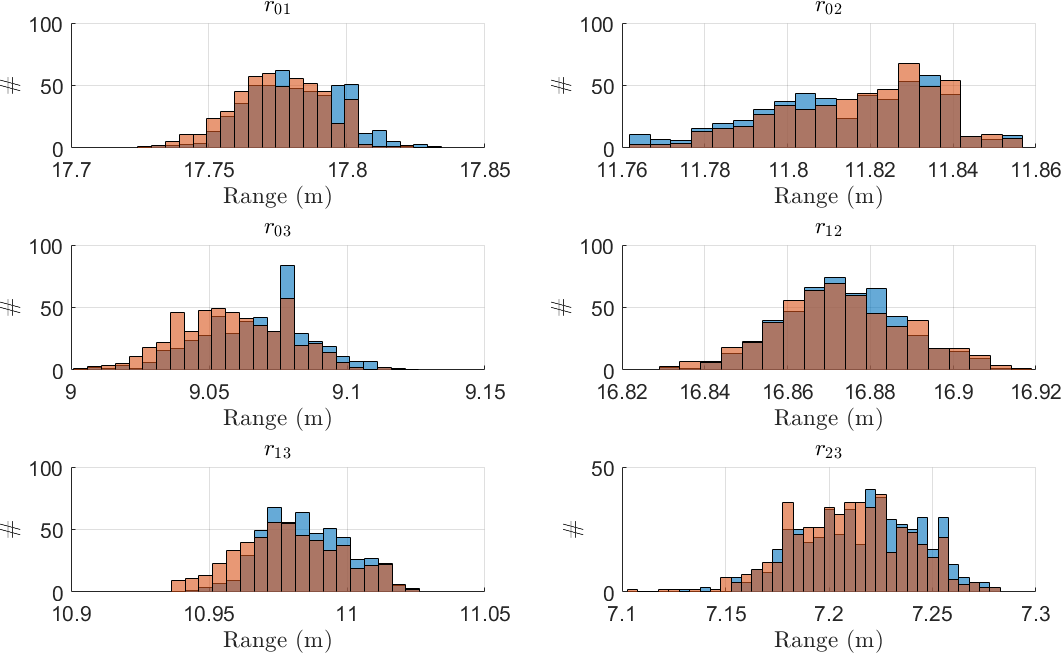
\includegraphics[scale=0.37]{autoranging.png}
  \end{center}
\end{frame}

\begin{frame}[shrink=10]{Nuova procedura di autoranging}
  Tenendo conto della simmetria la procedura diventa la seguente.
  \par
  Ogni ancora \alert{a turno} si comporta da ancora \alert{master}  ovvero:
  \begin{itemize}
  \item [1.] invia un messaggio di Poll a tutte le ancore \alert{non} master;
  \item [2.] legge nella risposta, di ciascuna ancora, il tof, lo trasforma in range espresso in metri e lo somma
    in una variabile necessaria per calcolare le medie successivamente;
  \item [3.] invia un messaggio di Final a tutte le ancore \alert{non} master nel quale specifica anche se ha terminato il suo compito
    di ancora master.
  \end{itemize}
  La procedura descritta nei precedenti punti viene ripetuta un numero di volte sufficiente ad ottenere almeno $M/2$ misure per
  ogni range di interesse. Si noti che lo scambio di messaggi Poll, Risposta, Final avviene con un meccanismo a divisione di tempi simile
  a quello utilizzato nella normale procedura di ranging.
\end{frame}

\begin{frame}[shrink = 10]{Nuova procedura di autoranging}
  Ogni ancora \alert{non} master:
  \begin{itemize}
  \item [1.] Ogni volta che riceve un messaggio di Poll da un ancora master risponde, quando è il proprio turno
    ossia sfruttando il solito meccanismo a divisione di tempi, inviando il tof calcolato nell'istanza precedente;
  \item [2.] Ogni volta che riceve un messaggio di Final da un ancora master calcola il nuovo tof. Inoltre,
    sfruttando il principio di simmetria precedentemente esposto, lo trasforma in range espresso in metri e lo somma
    in una variabile necessaria per calcolare le medie successivamente. Infine, se il messaggio di Final indica che l'ancora master
    ha terminato il proprio compito, l'ancora incrementa un contatore \lstinline!anchorRngMaster! che le consente di scoprire se è arrivato il proprio turno svolgere
    il ruolo di ancora master.
  \end{itemize}
\end{frame}

\begin{frame}{Termine della procedura di autoranging}
  Tutte le ancore, eccetto l'ultima, si rendono conto che l'intera procedura è terminata quando:
  \begin{itemize}
  \item [1.] ricevono il messaggio di Final dall'\alert{ultima} ancora master che indica che ha terminato il suo compito di ancora master;
  \item [2.] incrementano il contatore \lstinline!anchorRngMaster! e trovano che è pari al numero totale di ancore.
  \end{itemize}
  L'ultima ancora, ossia quella con l'indirizzo più alto, dato che non riceve il Final da nessun'altra ancora, esegue il controllo sul
  contatore nel momento in cui manda il suo ultimo messaggio di Final.
\end{frame}

\begin{frame}{Nuovi messaggi}
  Con l'aggiunta della procedura di autoranging alcuni messaggi, che erano utilizzati nella normale procedura di ranging, sono stati modificati
  ed altri sono stati aggiunti.
  I nuovi messaggi definiti per la procedura di autoranging sono:
  \begin{itemize}
  \item[-]\lstinline!RTLS_DEMO_MSG_ANCH_POLL! messaggio di Poll inviato dall'ancora \alert{master} durante la procedura di autoranging;
  \item[-]\lstinline!RTLS_DEMO_MSG_ANCH_FINAL! messaggio di Final inviato dall'ancora \alert{master} durante la procedura di autoranging;
  \item[-]\lstinline!RTLS_DEMO_MSG_ANCH_RESP2! messaggio di Risposta inviato dall'ancora \alert{non master} durante la procedura di autoranging.
  \end{itemize}
  Per completezza nelle slide successive viene riportata la struttura del campo \lstinline!msg_data! per tutti i tipi
  di messaggio.
\end{frame}

\begin{frame}{Messaggio di Poll - \lstinline!RTLS_DEMO_MSG_TAG_POLL!}
  \begin{center}
    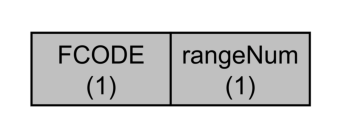
\includegraphics[height=3.4em]{message_f_tag_poll.pdf}
  \end{center}
  \begin{itemize}
  \item[-] \lstinline!FCODE = RTLS_DEMO_MSG_TAG_POLL!
  \item[-] \lstinline!rangeNum!: range number della trasmissione
  \end{itemize}
\end{frame}

\begin{frame}{Messaggio di Final - \lstinline!RTLS_DEMO_MSG_TAG_FINAL!}
  \begin{center}
    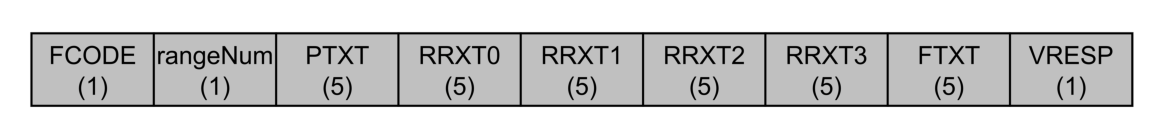
\includegraphics[height=3.4em]{message_f_tag_final.pdf}
  \end{center}
  \begin{itemize}
  \item[-] \lstinline!FCODE = RTLS_DEMO_MSG_TAG_FINAL!
  \item[-] \lstinline!rangeNum!: range number della trasmissione
  \item[-] \lstinline!PTXT!: tempo di invio del Poll
  \item[-] \lstinline!RRXT0!: tempo di ricezione della risposta da ancora 0
  \item[-] \lstinline!RRXT1!: tempo di ricezione della risposta da ancora 1
  \item[-] \lstinline!RRXT2!: tempo di ricezione della risposta da ancora 2
  \item[-] \lstinline!RRXT3!: tempo di ricezione della risposta da ancora 3
  \item[-] \lstinline!FTXT!: tempo di invio del Final
  \item[-] \lstinline!VRESP!: maschera della risposte valide ricevute
  \end{itemize}
\end{frame}

\begin{frame}{Messaggio di Risposta - \lstinline!RTLS_DEMO_MSG_ANCH_RESP!}
  \begin{center}
    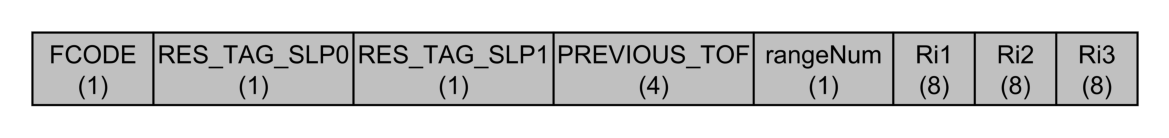
\includegraphics[height=3.4em]{message_f_anch_resp_new.pdf}
  \end{center}
  \begin{itemize}
  \item[-] \lstinline!FCODE = RTLS_DEMO_MSG_ANCH_RESP!
  \item[-] \lstinline!RES_TAG_SLP0!: parte alta dello sleep correction calcolato dall'ancora 0
  \item[-] \lstinline!RES_TAG_SLP1!: parte bassa dello sleep correction calcolato dall'ancora 0
  \item[-] \lstinline!PREVIOUS_TOF!: tof calcolato al passo precedente dall'ancora
  \item[-] \lstinline!rangeNum!: range number della trasmissione
  \item[-] \lstinline!Rij!: media dei range tra l'ancora $i$ e l'ancora $j$
  \end{itemize}
\end{frame}

\begin{frame}{Messaggio di Poll - \lstinline!RTLS_DEMO_MSG_ANCH_POLL!}
  \begin{center}
    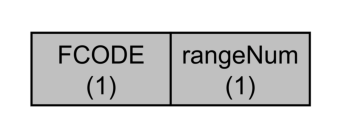
\includegraphics[height=3.4em]{message_f_tag_poll.pdf}
  \end{center}
  \begin{itemize}
  \item[-] \lstinline!FCODE = RTLS_DEMO_MSG_ANCH_POLL!
  \item[-] \lstinline!rangeNum!: range number della trasmissione
  \end{itemize}
\end{frame}

\begin{frame}{Messaggio di Final - \lstinline!RTLS_DEMO_MSG_ANCH_FINAL!}
  \begin{center}
    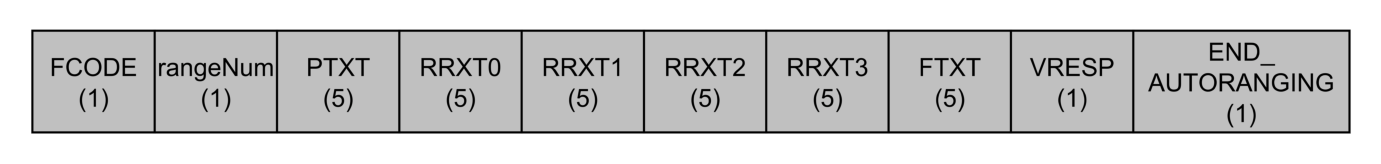
\includegraphics[height=3.4em]{message_f_anch_final.pdf}
  \end{center}
  \begin{itemize}
  \item[-] \lstinline!FCODE = RTLS_DEMO_MSG_ANCH_FINAL!
  \item[-] \lstinline!rangeNum!: range number della trasmissione
  \item[-] \lstinline!PTXT!: tempo di invio del Poll
  \item[-] \lstinline!RRXT0!: tempo di ricezione della risposta da ancora 0
  \item[-] \lstinline!RRXT1!: tempo di ricezione della risposta da ancora 1
  \item[-] \lstinline!RRXT2!: tempo di ricezione della risposta da ancora 2
  \item[-] \lstinline!RRXT3!: tempo di ricezione della risposta da ancora 3
  \item[-] \lstinline!FTXT!: tempo di invio del Final
  \item[-] \lstinline!VRESP!: maschera della risposte valide ricevute
  \item[-] \lstinline!END_AUTORANGING!: flag fine turno di ancora master
  \end{itemize}
\end{frame}

\begin{frame}{Messaggio di Risposta - \lstinline!RTLS_DEMO_MSG_ANCH_RESP2!}
  \begin{center}
    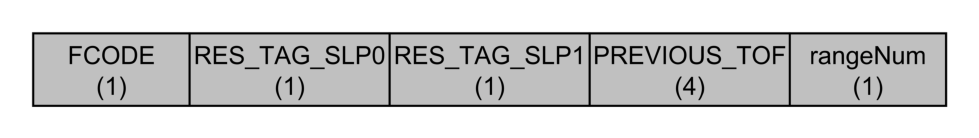
\includegraphics[height=3.4em]{message_f_anch_resp.pdf}
  \end{center}
  \begin{itemize}
  \item[-] \lstinline!FCODE = RTLS_DEMO_MSG_ANCH_RESP2!
  \item[-] \lstinline!RES_TAG_SLP0!: parte alta dello sleep correction calcolato dall'ancora 0
  \item[-] \lstinline!RES_TAG_SLP1!: parte bassa dello sleep correction calcolato dall'ancora 0
  \item[-] \lstinline!PREVIOUS_TOF!: tof calcolato al passo precedente dall'ancora
  \item[-] \lstinline!rangeNum!: range number della trasmissione
  \end{itemize}
  Durante la procedura di autoranging lo sleep correction non viene utilizzato poiché ogni ancora si comporta da master
  a turno e non può accadere che più ancore master trasmettano contemporaneamente.
\end{frame}

\begin{frame}{Maggiori informazioni}
  Per maggiori dettagli sull'intera procedura si rimanda:
  \begin{itemize}
  \item[-] ai diagrammi contenenti le macchine a stati ed i sequence diagram allegati al presente report;
  \item[-] alla guida al codice sviluppato (slides successive);
  \item[-] al codice sviluppato.
  \end{itemize}
\end{frame}
